\documentclass[tikz,border=8pt]{standalone}
\usepackage{lmodern}\usetikzlibrary{arrows.meta,positioning,fit,backgrounds}
\definecolor{rmit}{HTML}{E04B2A}\definecolor{aws}{HTML}{EAF2F8}\definecolor{optional}{HTML}{FFF1DE}
\tikzset{box/.style={draw,rounded corners,fill=aws,minimum width=27mm,minimum height=11mm,align=center,font=\sffamily\scriptsize},opt/.style={box,fill=optional},ext/.style={box,fill=black!5},edge/.style={-{Latex[length=1.8mm]},thick,font=\sffamily\tiny,align=center},async/.style={edge,dashed}}
\begin{document}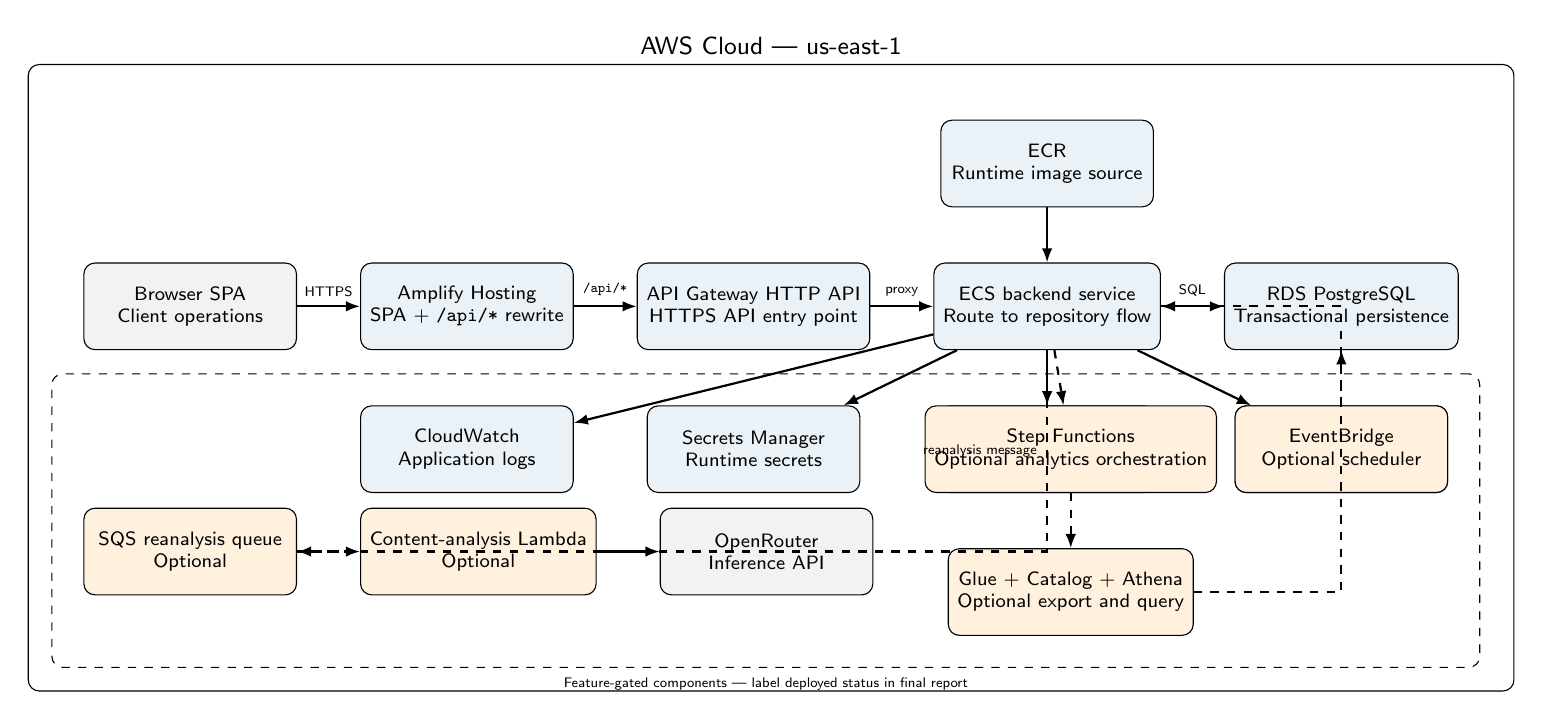
\begin{tikzpicture}[node distance=7mm and 8mm]
\node[ext] (browser) {Browser SPA\\Client operations};
\node[box,right=of browser] (amplify) {Amplify Hosting\\SPA + \texttt{/api/*} rewrite};
\node[box,right=of amplify] (api) {API Gateway HTTP API\\HTTPS API entry point};
\node[box,right=of api] (ecs) {ECS backend service\\Route to repository flow};
\node[box,below=of ecs] (ec2) {EC2 container instance\\ECS capacity};
\node[box,right=of ecs] (rds) {RDS PostgreSQL\\Transactional persistence};
\node[box,above=of ecs] (ecr) {ECR\\Runtime image source};
\node[box,below=of rds] (s3) {S3 media bucket\\Binary objects};
\node[box,below=of api] (secrets) {Secrets Manager\\Runtime secrets};
\node[box,below=of amplify] (logs) {CloudWatch\\Application logs};
\node[opt,below=20mm of browser] (sqs) {SQS reanalysis queue\\Optional};
\node[opt,right=of sqs] (lambda) {Content-analysis Lambda\\Optional};
\node[ext,right=of lambda] (openrouter) {OpenRouter\\Inference API};
\node[opt,below=of ecs,xshift=3mm] (sfn) {Step Functions\\Optional analytics orchestration};
\node[opt,below=of sfn] (glue) {Glue + Catalog + Athena\\Optional export and query};
\node[opt,below=of rds] (event) {EventBridge\\Optional scheduler};
\draw[edge] (browser) -- node[above]{HTTPS} (amplify);\draw[edge] (amplify) -- node[above]{\texttt{/api/*}} (api);\draw[edge] (api) -- node[above]{proxy} (ecs);\draw[edge] (ecs) -- node[above]{SQL} (rds);\draw[edge] (ecr) -- (ecs);\draw[edge] (ecs) -- (s3);\draw[edge] (ecs) -- (secrets);\draw[edge] (ecs) -- (logs);\draw[edge] (ecs) -- (ec2);
\draw[async] (ecs) |- node[pos=.25,left]{reanalysis message} (sqs);\draw[async] (sqs) -- (lambda);\draw[edge] (lambda) -- (openrouter);\draw[async] (ecs) -- (sfn);\draw[async] (event) |- (ecs);\draw[async] (sfn) -- (glue);\draw[async] (glue) -| (rds);
\begin{scope}[on background layer]\node[draw,rounded corners,fit=(amplify)(api)(ecs)(rds)(s3)(ecr)(secrets)(logs)(ec2)(sqs)(lambda)(sfn)(glue)(event),inner sep=7mm,label={[font=\sffamily\small]above:AWS Cloud --- us-east-1}] {};\node[draw,dashed,rounded corners,fit=(sqs)(lambda)(sfn)(glue)(event),inner sep=4mm,label={[font=\sffamily\tiny]below:Feature-gated components --- label deployed status in final report}] {};\end{scope}
\end{tikzpicture}\end{document}
